\documentclass{standalone}
\usepackage{tikz}
\usetikzlibrary{patterns, positioning}


\begin{document}
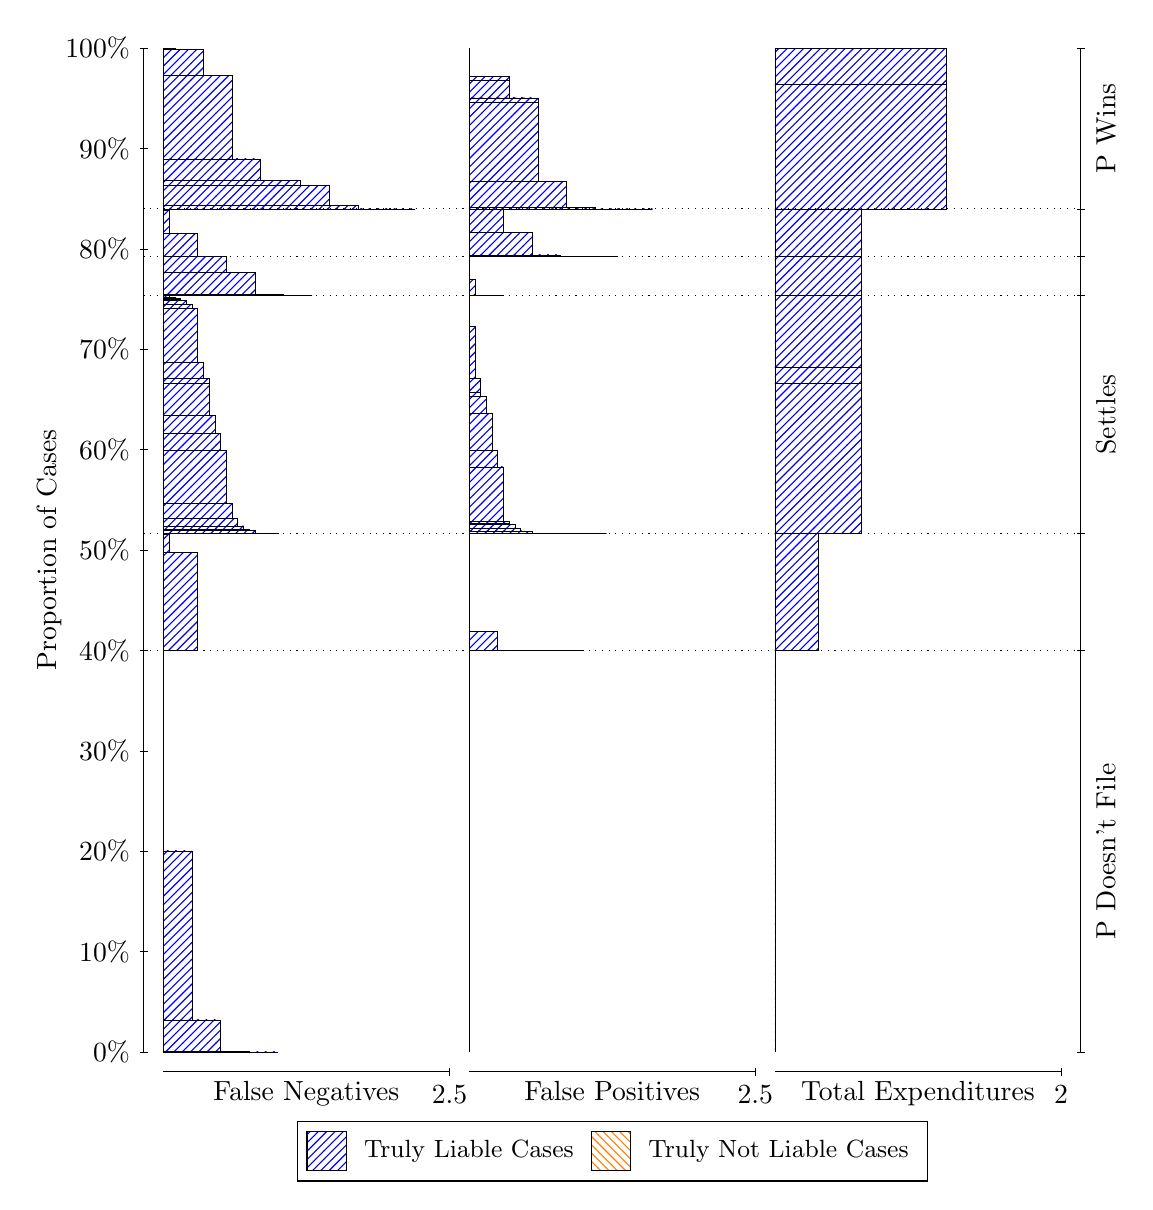
\begin{tikzpicture}
\draw[black, very thin] (1.5,1.75) -- (1.5,14.5);
\node[rotate=90, text=black, anchor=center] at (0.3, 8.125) {Proportion of Cases};
\draw[black, very thin] (1.45,1.75) -- (1.55,1.75);
\node[text=black, anchor=east] at (1.45, 1.75) {0\%};
\draw[black, very thin] (1.45,3.025) -- (1.55,3.025);
\node[text=black, anchor=east] at (1.45, 3.025) {10\%};
\draw[black, very thin] (1.45,4.3) -- (1.55,4.3);
\node[text=black, anchor=east] at (1.45, 4.3) {20\%};
\draw[black, very thin] (1.45,5.575) -- (1.55,5.575);
\node[text=black, anchor=east] at (1.45, 5.575) {30\%};
\draw[black, very thin] (1.45,6.85) -- (1.55,6.85);
\node[text=black, anchor=east] at (1.45, 6.85) {40\%};
\draw[black, very thin] (1.45,8.125) -- (1.55,8.125);
\node[text=black, anchor=east] at (1.45, 8.125) {50\%};
\draw[black, very thin] (1.45,9.4) -- (1.55,9.4);
\node[text=black, anchor=east] at (1.45, 9.4) {60\%};
\draw[black, very thin] (1.45,10.675) -- (1.55,10.675);
\node[text=black, anchor=east] at (1.45, 10.675) {70\%};
\draw[black, very thin] (1.45,11.95) -- (1.55,11.95);
\node[text=black, anchor=east] at (1.45, 11.95) {80\%};
\draw[black, very thin] (1.45,13.225) -- (1.55,13.225);
\node[text=black, anchor=east] at (1.45, 13.225) {90\%};
\draw[black, very thin] (1.45,14.5) -- (1.55,14.5);
\node[text=black, anchor=east] at (1.45, 14.5) {100\%};

\draw[black, very thin] (13.4,1.75) -- (13.4,14.5);
\draw[black, very thin] (13.35,1.75) -- (13.45,1.75);
\node[anchor=west] at (13.35, 1.75) {};
\draw[black, very thin] (13.35,6.8489) -- (13.45,6.8489);
\node[anchor=west] at (13.35, 6.8489) {};
\draw[black, very thin] (13.35,8.3327) -- (13.45,8.3327);
\node[anchor=west] at (13.35, 8.3327) {};
\draw[black, very thin] (13.35,11.358) -- (13.45,11.358);
\node[anchor=west] at (13.35, 11.358) {};
\draw[black, very thin] (13.35,11.855) -- (13.45,11.855);
\node[anchor=west] at (13.35, 11.855) {};
\draw[black, very thin] (13.35,12.458) -- (13.45,12.458);
\node[anchor=west] at (13.35, 12.458) {};
\draw[black, very thin] (13.35,14.5) -- (13.45,14.5);
\node[anchor=west] at (13.35, 14.5) {};

\draw[black, very thin, pattern color=blue, pattern=north east lines] (1.75,1.75) rectangle (3.2033,1.75);
\draw[black, very thin, pattern color=blue, pattern=north east lines] (1.75,1.75) rectangle (2.84,1.7534);
\draw[black, very thin, pattern color=blue, pattern=north east lines] (1.75,1.7534) rectangle (2.4767,2.158);
\draw[black, very thin, pattern color=blue, pattern=north east lines] (1.75,2.158) rectangle (2.1133,4.3029);
\draw[black, very thin, pattern color=orange, pattern=north west lines] (1.75,4.3029) rectangle (1.75,4.3029);
\draw[black, very thin, pattern color=blue, pattern=north east lines] (1.75,4.3029) rectangle (1.75,6.8489);
\draw[black, very thin, pattern color=blue, pattern=north east lines] (1.75,6.8489) rectangle (2.186,8.0903);
\draw[black, very thin, pattern color=blue, pattern=north east lines] (1.75,8.0903) rectangle (1.8227,8.331);
\draw[black, very thin, pattern color=orange, pattern=north west lines] (1.75,8.331) rectangle (1.75,8.331);
\draw[black, very thin, pattern color=blue, pattern=north east lines] (1.75,8.331) rectangle (1.75,8.3327);
\draw[black, very thin, pattern color=blue, pattern=north east lines] (1.75,8.3327) rectangle (3.2033,8.3328);
\draw[black, very thin, pattern color=blue, pattern=north east lines] (1.75,8.3328) rectangle (3.058,8.3331);
\draw[black, very thin, pattern color=blue, pattern=north east lines] (1.75,8.3331) rectangle (2.9127,8.3767);
\draw[black, very thin, pattern color=blue, pattern=north east lines] (1.75,8.3767) rectangle (2.84,8.3891);
\draw[black, very thin, pattern color=blue, pattern=north east lines] (1.75,8.3891) rectangle (2.7673,8.4306);
\draw[black, very thin, pattern color=blue, pattern=north east lines] (1.75,8.4306) rectangle (2.6947,8.529);
\draw[black, very thin, pattern color=blue, pattern=north east lines] (1.75,8.529) rectangle (2.622,8.7208);
\draw[black, very thin, pattern color=blue, pattern=north east lines] (1.75,8.7208) rectangle (2.5493,9.3866);
\draw[black, very thin, pattern color=blue, pattern=north east lines] (1.75,9.3866) rectangle (2.4767,9.6102);
\draw[black, very thin, pattern color=blue, pattern=north east lines] (1.75,9.6102) rectangle (2.404,9.8314);
\draw[black, very thin, pattern color=blue, pattern=north east lines] (1.75,9.8314) rectangle (2.3313,10.237);
\draw[black, very thin, pattern color=blue, pattern=north east lines] (1.75,10.237) rectangle (2.3313,10.3);
\draw[black, very thin, pattern color=blue, pattern=north east lines] (1.75,10.3) rectangle (2.2587,10.509);
\draw[black, very thin, pattern color=blue, pattern=north east lines] (1.75,10.509) rectangle (2.186,11.198);
\draw[black, very thin, pattern color=blue, pattern=north east lines] (1.75,11.198) rectangle (2.1133,11.244);
\draw[black, very thin, pattern color=blue, pattern=north east lines] (1.75,11.244) rectangle (2.0407,11.295);
\draw[black, very thin, pattern color=blue, pattern=north east lines] (1.75,11.295) rectangle (1.968,11.313);
\draw[black, very thin, pattern color=blue, pattern=north east lines] (1.75,11.313) rectangle (1.968,11.321);
\draw[black, very thin, pattern color=blue, pattern=north east lines] (1.75,11.321) rectangle (1.8953,11.333);
\draw[black, very thin, pattern color=blue, pattern=north east lines] (1.75,11.333) rectangle (1.8227,11.357);
\draw[black, very thin, pattern color=orange, pattern=north west lines] (1.75,11.357) rectangle (1.75,11.357);
\draw[black, very thin, pattern color=blue, pattern=north east lines] (1.75,11.357) rectangle (1.75,11.358);
\draw[black, very thin, pattern color=blue, pattern=north east lines] (1.75,11.358) rectangle (3.6393,11.358);
\draw[black, very thin, pattern color=blue, pattern=north east lines] (1.75,11.358) rectangle (3.276,11.37);
\draw[black, very thin, pattern color=blue, pattern=north east lines] (1.75,11.37) rectangle (2.9127,11.653);
\draw[black, very thin, pattern color=blue, pattern=north east lines] (1.75,11.653) rectangle (2.5493,11.853);
\draw[black, very thin, pattern color=blue, pattern=north east lines] (1.75,11.853) rectangle (2.186,11.855);
\draw[black, very thin, pattern color=orange, pattern=north west lines] (1.75,11.855) rectangle (1.75,11.855);
\draw[black, very thin, pattern color=blue, pattern=north east lines] (1.75,11.855) rectangle (2.186,12.15);
\draw[black, very thin, pattern color=blue, pattern=north east lines] (1.75,12.15) rectangle (1.8227,12.441);
\draw[black, very thin, pattern color=orange, pattern=north west lines] (1.75,12.441) rectangle (1.75,12.441);
\draw[black, very thin, pattern color=blue, pattern=north east lines] (1.75,12.441) rectangle (1.75,12.458);
\draw[black, very thin, pattern color=blue, pattern=north east lines] (1.75,12.458) rectangle (4.9473,12.458);
\draw[black, very thin, pattern color=blue, pattern=north east lines] (1.75,12.458) rectangle (4.584,12.458);
\draw[black, very thin, pattern color=blue, pattern=north east lines] (1.75,12.458) rectangle (4.2207,12.501);
\draw[black, very thin, pattern color=blue, pattern=north east lines] (1.75,12.501) rectangle (3.8573,12.753);
\draw[black, very thin, pattern color=blue, pattern=north east lines] (1.75,12.753) rectangle (3.712,12.753);
\draw[black, very thin, pattern color=blue, pattern=north east lines] (1.75,12.753) rectangle (3.494,12.817);
\draw[black, very thin, pattern color=blue, pattern=north east lines] (1.75,12.817) rectangle (3.3487,12.822);
\draw[black, very thin, pattern color=blue, pattern=north east lines] (1.75,12.822) rectangle (3.1307,12.822);
\draw[black, very thin, pattern color=blue, pattern=north east lines] (1.75,12.822) rectangle (2.9853,13.092);
\draw[black, very thin, pattern color=blue, pattern=north east lines] (1.75,13.092) rectangle (2.7673,13.092);
\draw[black, very thin, pattern color=blue, pattern=north east lines] (1.75,13.092) rectangle (2.622,14.154);
\draw[black, very thin, pattern color=blue, pattern=north east lines] (1.75,14.154) rectangle (2.2587,14.485);
\draw[black, very thin, pattern color=blue, pattern=north east lines] (1.75,14.485) rectangle (1.8953,14.5);
\draw[black, very thin, pattern color=orange, pattern=north west lines] (1.75,14.5) rectangle (1.75,14.5);
\draw[black, very thin, pattern color=blue, pattern=north east lines] (1.75,14.5) rectangle (1.75,14.5);
\draw[black, very thin, pattern color=orange, pattern=north west lines] (5.6333,1.75) rectangle (5.6333,1.75);
\draw[black, very thin, pattern color=blue, pattern=north east lines] (5.6333,1.75) rectangle (5.6333,6.8489);
\draw[black, very thin, pattern color=orange, pattern=north west lines] (5.6333,6.8489) rectangle (7.0867,6.8489);
\draw[black, very thin, pattern color=blue, pattern=north east lines] (5.6333,6.8489) rectangle (7.0867,6.8489);
\draw[black, very thin, pattern color=blue, pattern=north east lines] (5.6333,6.8489) rectangle (6.7233,6.8489);
\draw[black, very thin, pattern color=blue, pattern=north east lines] (5.6333,6.8489) rectangle (6.36,6.8506);
\draw[black, very thin, pattern color=blue, pattern=north east lines] (5.6333,6.8506) rectangle (5.9967,7.0913);
\draw[black, very thin, pattern color=blue, pattern=north east lines] (5.6333,7.0913) rectangle (5.6333,8.3327);
\draw[black, very thin, pattern color=orange, pattern=north west lines] (5.6333,8.3327) rectangle (7.3773,8.3327);
\draw[black, very thin, pattern color=blue, pattern=north east lines] (5.6333,8.3327) rectangle (7.3773,8.3327);
\draw[black, very thin, pattern color=orange, pattern=north west lines] (5.6333,8.3327) rectangle (7.232,8.3327);
\draw[black, very thin, pattern color=blue, pattern=north east lines] (5.6333,8.3327) rectangle (7.232,8.3327);
\draw[black, very thin, pattern color=orange, pattern=north west lines] (5.6333,8.3327) rectangle (7.0867,8.3327);
\draw[black, very thin, pattern color=blue, pattern=north east lines] (5.6333,8.3327) rectangle (7.0867,8.3327);
\draw[black, very thin, pattern color=blue, pattern=north east lines] (5.6333,8.3327) rectangle (7.014,8.3327);
\draw[black, very thin, pattern color=orange, pattern=north west lines] (5.6333,8.3327) rectangle (6.9413,8.3327);
\draw[black, very thin, pattern color=blue, pattern=north east lines] (5.6333,8.3327) rectangle (6.9413,8.3327);
\draw[black, very thin, pattern color=blue, pattern=north east lines] (5.6333,8.3327) rectangle (6.8687,8.3327);
\draw[black, very thin, pattern color=orange, pattern=north west lines] (5.6333,8.3327) rectangle (6.796,8.3327);
\draw[black, very thin, pattern color=blue, pattern=north east lines] (5.6333,8.3327) rectangle (6.796,8.3327);
\draw[black, very thin, pattern color=blue, pattern=north east lines] (5.6333,8.3327) rectangle (6.7233,8.3327);
\draw[black, very thin, pattern color=orange, pattern=north west lines] (5.6333,8.3327) rectangle (6.6507,8.3327);
\draw[black, very thin, pattern color=blue, pattern=north east lines] (5.6333,8.3327) rectangle (6.6507,8.3328);
\draw[black, very thin, pattern color=blue, pattern=north east lines] (5.6333,8.3328) rectangle (6.578,8.3329);
\draw[black, very thin, pattern color=blue, pattern=north east lines] (5.6333,8.3329) rectangle (6.5053,8.3336);
\draw[black, very thin, pattern color=orange, pattern=north west lines] (5.6333,8.3336) rectangle (6.5053,8.3336);
\draw[black, very thin, pattern color=blue, pattern=north east lines] (5.6333,8.3336) rectangle (6.5053,8.3336);
\draw[black, very thin, pattern color=blue, pattern=north east lines] (5.6333,8.3336) rectangle (6.4327,8.3576);
\draw[black, very thin, pattern color=blue, pattern=north east lines] (5.6333,8.3576) rectangle (6.36,8.369);
\draw[black, very thin, pattern color=blue, pattern=north east lines] (5.6333,8.369) rectangle (6.2873,8.3951);
\draw[black, very thin, pattern color=blue, pattern=north east lines] (5.6333,8.3951) rectangle (6.2147,8.446);
\draw[black, very thin, pattern color=blue, pattern=north east lines] (5.6333,8.446) rectangle (6.142,8.468);
\draw[black, very thin, pattern color=blue, pattern=north east lines] (5.6333,8.468) rectangle (6.142,8.4921);
\draw[black, very thin, pattern color=blue, pattern=north east lines] (5.6333,8.4921) rectangle (6.0693,9.1812);
\draw[black, very thin, pattern color=blue, pattern=north east lines] (5.6333,9.1812) rectangle (5.9967,9.3899);
\draw[black, very thin, pattern color=blue, pattern=north east lines] (5.6333,9.3899) rectangle (5.924,9.8589);
\draw[black, very thin, pattern color=blue, pattern=north east lines] (5.6333,9.8589) rectangle (5.8513,10.08);
\draw[black, very thin, pattern color=blue, pattern=north east lines] (5.6333,10.08) rectangle (5.7787,10.132);
\draw[black, very thin, pattern color=blue, pattern=north east lines] (5.6333,10.132) rectangle (5.7787,10.304);
\draw[black, very thin, pattern color=blue, pattern=north east lines] (5.6333,10.304) rectangle (5.706,10.969);
\draw[black, very thin, pattern color=blue, pattern=north east lines] (5.6333,10.969) rectangle (5.6333,11.358);
\draw[black, very thin, pattern color=orange, pattern=north west lines] (5.6333,11.358) rectangle (6.0693,11.358);
\draw[black, very thin, pattern color=blue, pattern=north east lines] (5.6333,11.358) rectangle (6.0693,11.36);
\draw[black, very thin, pattern color=blue, pattern=north east lines] (5.6333,11.36) rectangle (5.706,11.56);
\draw[black, very thin, pattern color=blue, pattern=north east lines] (5.6333,11.56) rectangle (5.6333,11.855);
\draw[black, very thin, pattern color=orange, pattern=north west lines] (5.6333,11.855) rectangle (7.5227,11.855);
\draw[black, very thin, pattern color=blue, pattern=north east lines] (5.6333,11.855) rectangle (7.5227,11.855);
\draw[black, very thin, pattern color=blue, pattern=north east lines] (5.6333,11.855) rectangle (7.1593,11.855);
\draw[black, very thin, pattern color=blue, pattern=north east lines] (5.6333,11.855) rectangle (6.796,11.872);
\draw[black, very thin, pattern color=blue, pattern=north east lines] (5.6333,11.872) rectangle (6.4327,12.163);
\draw[black, very thin, pattern color=blue, pattern=north east lines] (5.6333,12.163) rectangle (6.0693,12.458);
\draw[black, very thin, pattern color=orange, pattern=north west lines] (5.6333,12.458) rectangle (7.9587,12.458);
\draw[black, very thin, pattern color=blue, pattern=north east lines] (5.6333,12.458) rectangle (7.9587,12.458);
\draw[black, very thin, pattern color=orange, pattern=north west lines] (5.6333,12.458) rectangle (7.5953,12.458);
\draw[black, very thin, pattern color=blue, pattern=north east lines] (5.6333,12.458) rectangle (7.5953,12.458);
\draw[black, very thin, pattern color=orange, pattern=north west lines] (5.6333,12.458) rectangle (7.232,12.458);
\draw[black, very thin, pattern color=blue, pattern=north east lines] (5.6333,12.458) rectangle (7.232,12.473);
\draw[black, very thin, pattern color=blue, pattern=north east lines] (5.6333,12.473) rectangle (6.8687,12.804);
\draw[black, very thin, pattern color=orange, pattern=north west lines] (5.6333,12.804) rectangle (6.8687,12.804);
\draw[black, very thin, pattern color=blue, pattern=north east lines] (5.6333,12.804) rectangle (6.8687,12.804);
\draw[black, very thin, pattern color=blue, pattern=north east lines] (5.6333,12.804) rectangle (6.5053,13.805);
\draw[black, very thin, pattern color=blue, pattern=north east lines] (5.6333,13.805) rectangle (6.5053,13.866);
\draw[black, very thin, pattern color=orange, pattern=north west lines] (5.6333,13.866) rectangle (6.36,13.866);
\draw[black, very thin, pattern color=blue, pattern=north east lines] (5.6333,13.866) rectangle (6.36,13.866);
\draw[black, very thin, pattern color=blue, pattern=north east lines] (5.6333,13.866) rectangle (6.142,14.093);
\draw[black, very thin, pattern color=blue, pattern=north east lines] (5.6333,14.093) rectangle (6.142,14.136);
\draw[black, very thin, pattern color=orange, pattern=north west lines] (5.6333,14.136) rectangle (5.9967,14.136);
\draw[black, very thin, pattern color=blue, pattern=north east lines] (5.6333,14.136) rectangle (5.9967,14.136);
\draw[black, very thin, pattern color=blue, pattern=north east lines] (5.6333,14.136) rectangle (5.7787,14.14);
\draw[black, very thin, pattern color=blue, pattern=north east lines] (5.6333,14.14) rectangle (5.7787,14.141);
\draw[black, very thin, pattern color=orange, pattern=north west lines] (5.6333,14.141) rectangle (5.6333,14.141);
\draw[black, very thin, pattern color=blue, pattern=north east lines] (5.6333,14.141) rectangle (5.6333,14.5);
\draw[black, very thin, pattern color=orange, pattern=north west lines] (9.5167,1.75) rectangle (9.5167,1.75);
\draw[black, very thin, pattern color=blue, pattern=north east lines] (9.5167,1.75) rectangle (9.5167,6.8489);
\draw[black, very thin, pattern color=orange, pattern=north west lines] (9.5167,6.8489) rectangle (10.062,6.8489);
\draw[black, very thin, pattern color=blue, pattern=north east lines] (9.5167,6.8489) rectangle (10.062,8.3327);
\draw[black, very thin, pattern color=orange, pattern=north west lines] (9.5167,8.3327) rectangle (10.607,8.3327);
\draw[black, very thin, pattern color=blue, pattern=north east lines] (9.5167,8.3327) rectangle (10.607,10.241);
\draw[black, very thin, pattern color=orange, pattern=north west lines] (9.5167,10.241) rectangle (10.607,10.241);
\draw[black, very thin, pattern color=blue, pattern=north east lines] (9.5167,10.241) rectangle (10.607,10.45);
\draw[black, very thin, pattern color=orange, pattern=north west lines] (9.5167,10.45) rectangle (10.607,10.45);
\draw[black, very thin, pattern color=blue, pattern=north east lines] (9.5167,10.45) rectangle (10.607,11.358);
\draw[black, very thin, pattern color=orange, pattern=north west lines] (9.5167,11.358) rectangle (10.607,11.358);
\draw[black, very thin, pattern color=blue, pattern=north east lines] (9.5167,11.358) rectangle (10.607,11.855);
\draw[black, very thin, pattern color=orange, pattern=north west lines] (9.5167,11.855) rectangle (10.607,11.855);
\draw[black, very thin, pattern color=blue, pattern=north east lines] (9.5167,11.855) rectangle (10.607,12.458);
\draw[black, very thin, pattern color=orange, pattern=north west lines] (9.5167,12.458) rectangle (11.697,12.458);
\draw[black, very thin, pattern color=blue, pattern=north east lines] (9.5167,12.458) rectangle (11.697,14.036);
\draw[black, very thin, pattern color=orange, pattern=north west lines] (9.5167,14.036) rectangle (11.697,14.036);
\draw[black, very thin, pattern color=blue, pattern=north east lines] (9.5167,14.036) rectangle (11.697,14.5);
\draw[black, dotted] (1.5,6.8489) -- (13.4,6.8489);
\draw[black, dotted] (1.5,8.3327) -- (13.4,8.3327);
\draw[black, dotted] (1.5,11.358) -- (13.4,11.358);
\draw[black, dotted] (1.5,11.855) -- (13.4,11.855);
\draw[black, dotted] (1.5,12.458) -- (13.4,12.458);
\draw[black, very thin] (1.75,1.5) -- (5.3833,1.5);
\node[text=black, anchor=north] at (3.5667, 1.5) {False Negatives};
\draw[black, very thin] (5.3833,1.45) -- (5.3833,1.55);
\node[text=black, anchor=north] at (5.3833, 1.45) {2.5};

\draw[black, very thin] (5.6333,1.5) -- (9.2667,1.5);
\node[text=black, anchor=north] at (7.45, 1.5) {False Positives};
\draw[black, very thin] (9.2667,1.45) -- (9.2667,1.55);
\node[text=black, anchor=north] at (9.2667, 1.45) {2.5};

\draw[black, very thin] (9.5167,1.5) -- (13.15,1.5);
\node[text=black, anchor=north] at (11.333, 1.5) {Total Expenditures};
\draw[black, very thin] (13.15,1.45) -- (13.15,1.55);
\node[text=black, anchor=north] at (13.15, 1.45) {2};

\node[text=black, centered, rotate=90] at (13.72, 4.2994) {P Doesn't File};

\node[text=black, centered, rotate=90] at (13.72, 9.8451) {Settles};


\node[text=black, centered, rotate=90] at (13.72, 13.479) {P Wins};

\draw (7.449999999999999,1.5) node[draw=none] (baseCoordinate) {};
\begin{scope}[align=center]
        \matrix[scale=0.5, draw=black, below=0.5cm of baseCoordinate, nodes={draw}, column sep=0.1cm]{
            \node[rectangle, draw, minimum width=0.5cm, minimum height=0.5cm, pattern color=blue, pattern=north east lines] {}; &
            \node[draw=none, font=\small, text=black] (B) {Truly Liable Cases}; &
            \node[rectangle, draw, minimum width=0.5cm, minimum height=0.5cm, pattern color=orange, pattern=north west lines] {}; &
            \node[draw=none, font=\small, text=black] (B) {Truly Not Liable Cases}; \\
            };
\end{scope}

\end{tikzpicture}
\end{document}